\section{Method}

MorphoCLIP has image and text encoders trained with a contrastive text objective and optional replicate and plate-offset terms. The image encoder turns a well of five-channel Cell Painting sites into a 512-dimensional unit vector. The text encoder does the same for a prompt that describes the perturbation. Figure~\ref{fig:architecture} shows the pipeline.

\begin{figure*}[t]
    \centering
    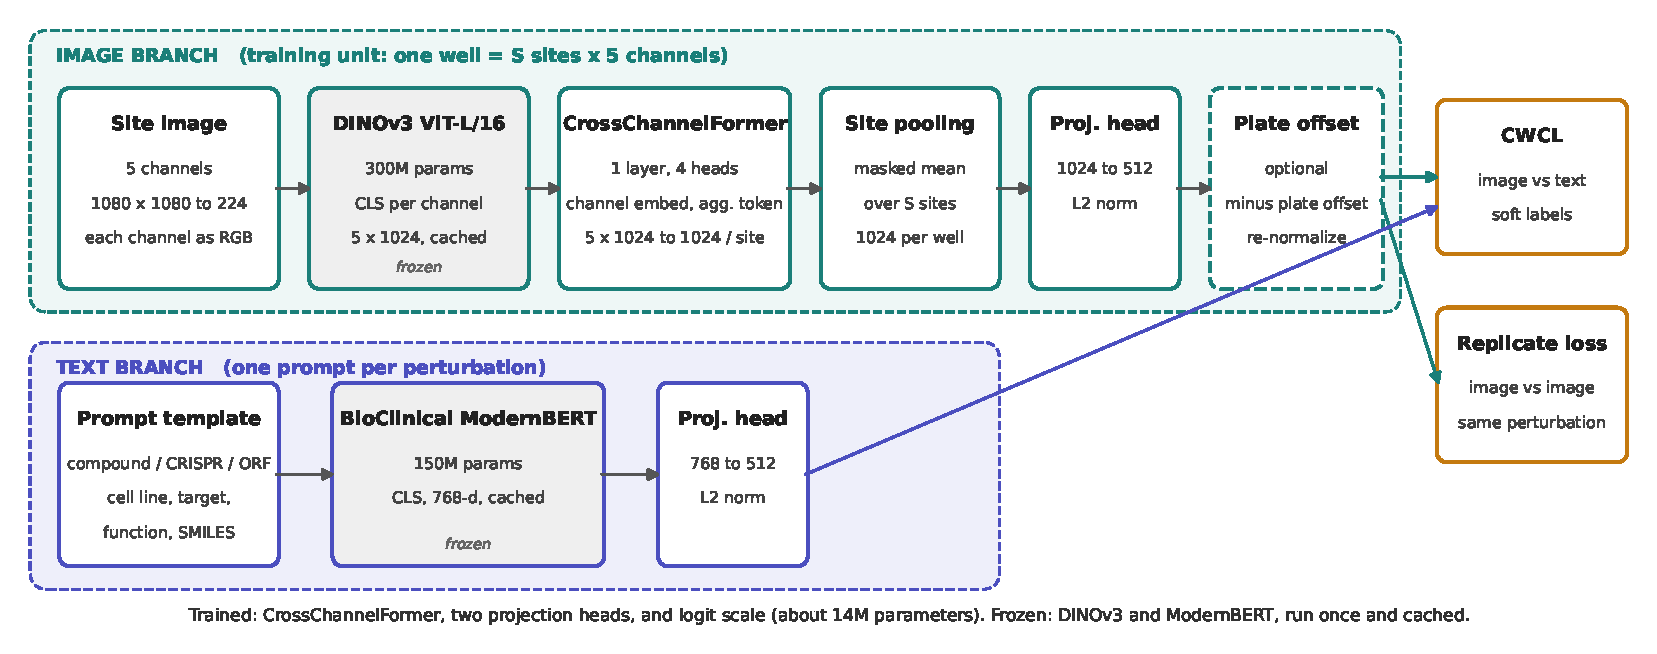
\includegraphics[width=\textwidth]{figures/architecture.pdf}
    \caption{MorphoCLIP. Each fluorescence channel of a site is encoded on its own by a frozen DINOv3 ViT-L/16, giving five 1024-d CLS tokens. A one-layer CrossChannelFormer attends over the five channel tokens and a learned aggregation token, and the aggregation token's output is the site vector. Site vectors are mean-pooled into a well vector and projected to the shared 512-d space. The prompt is encoded by a frozen BioClinical ModernBERT and projected to the same space. When plate offsets are on, the image embedding is shifted by its plate's offset and re-normalized before the losses. The trainable components are the CrossChannelFormer, the two projection heads and one logit-scale scalar, about 14M parameters in total.}
    \label{fig:architecture}
\end{figure*}

\subsection{Image Encoder}

A Cell Painting site has five fluorescence channels (Table~\ref{tab:channels}). We encode each channel on its own: the single-channel image is resized to the Hugging Face processor's native $224 \times 224$ input, copied to three channels, normalized with the processor statistics, and passed through a frozen DINOv3 ViT-L/16~\cite{simeoni2025dinov3} (300M parameters). The result is five 1024-dimensional CLS tokens per site,
\begin{equation}
    \{\mathbf{z}_c\}_{c=1}^{5}, \quad \mathbf{z}_c \in \mathbb{R}^{1024}.
\end{equation}

\begin{table}[t]
\centering
\caption{Cell Painting fluorescence channels used in MorphoCLIP.}
\label{tab:channels}
\begin{tabular}{@{}cll@{}}
\toprule
Ch & Stain & Target \\
\midrule
1 & MitoTracker / Alexa 647 & Mitochondria \\
2 & Phalloidin / Alexa 568 & Actin \\
3 & WGA / Alexa 488 & Golgi / plasma membrane \\
4 & Concanavalin A / Alexa 488 & Endoplasmic reticulum \\
5 & Hoechst 33342 & DNA / nucleus \\
\bottomrule
\end{tabular}
\end{table}

We use DINOv3 ViT-L rather than the larger DINOv2-g backbone used by CellCLIP. The channel tokens are written to disk once, and every training run reads from that cache. The backbone never runs during training.

\paragraph{CrossChannelFormer (CCF).} A one-layer transformer encoder~\cite{vaswani2017attention} with 4 heads merges the five channel tokens into one site vector, following the channel-aware design of CellCLIP~\cite{lu2025cellclip} and Channel ViT~\cite{bao2024channelvit}. Each token is L2-normalized so the five channels enter at a common scale, then a learned channel embedding $\mathbf{e}_c$ is added so the transformer can tell the stains apart. A learned aggregation token $\mathbf{q}$ is prepended and its output is the site vector:
\begin{equation}
    \mathbf{h}_{\text{site}} = \bigl[\,\text{CCF}\bigl(\mathbf{q},\, \hat{\mathbf{z}}_1 + \mathbf{e}_1,\, \dots,\, \hat{\mathbf{z}}_5 + \mathbf{e}_5\bigr)\,\bigr]_{0}, \quad \hat{\mathbf{z}}_c = \mathbf{z}_c / \|\mathbf{z}_c\|_2 .
\end{equation}
The layer is pre-norm with a feed-forward width of 4096 and GELU activations. The transformer can read out joint patterns across stains, for example a change that shows in both the mitochondrial and the ER channel. The CCF holds 12.6M of the 14M trained parameters.

\paragraph{Site-to-well pooling.} The training unit is a well. Site vectors are averaged under a site mask, so wells with 7, 9 or 16 imaged sites all produce one vector and the order of sites does not matter.

\paragraph{Image projection head.} A two-layer MLP with LayerNorm, GELU and dropout ($p = 0.3$) maps the well vector $\mathbf{h}_{\text{img}}$ to the shared space:
\begin{equation}
    f_{\text{img}}(\mathbf{x}) = \text{L2Norm}\bigl(\mathbf{W}_2\, \text{Drop}(\text{GELU}(\text{LN}(\mathbf{W}_1 \mathbf{h}_{\text{img}})))\bigr),
\end{equation}
with $\mathbf{W}_1 \in \mathbb{R}^{512 \times 1024}$ and $\mathbf{W}_2 \in \mathbb{R}^{512 \times 512}$.

\subsection{Text Encoder}

Each perturbation gets one prompt, built from CPJUMP1 metadata and external annotations with one of four templates:

\begin{itemize}
    \item \textbf{Compound:} \textit{``Cell Painting morphological profile of \{cell\_line\} cells treated with the compound \{compound\_name\}. Chemical structure (SMILES): \{smiles\}. Known target gene: \{target\_gene\}. Target protein function: \{gene\_function\}. Perturbation modality: chemical compound.''}
    \item \textbf{CRISPR:} \textit{``\dots\ with CRISPR-Cas9 knockout of gene \{gene\_symbol\}. Gene description: \{gene\_description\}. Gene function: \{gene\_function\}. Perturbation modality: CRISPR knockout.''}
    \item \textbf{ORF:} \textit{``\dots\ overexpressing gene \{gene\_symbol\} via open reading frame construct. Gene description: \{gene\_description\}. Gene function: \{gene\_function\}. Perturbation modality: ORF overexpression.''}
    \item \textbf{Negative control:} \textit{``\dots\ treated with DMSO vehicle control. No active perturbation applied.''}
\end{itemize}

Missing fields become ``unknown''. Compound annotations come from ChEMBL and the CPJUMP1 metadata. Gene descriptions and functions come from UniProt. Prompts are keyed by the perturbation identifier (\texttt{broad\_sample}), so replicate wells of one perturbation share one text vector.

We encode each prompt with a frozen BioClinical ModernBERT~\cite{sounack2025bioclinical} (150M parameters, 768-d CLS token). A trainable projection head with the same shape as the image head maps the CLS token to the shared space:
\begin{equation}
    f_{\text{txt}}(t) = \text{L2Norm}\bigl(\mathbf{W}_4\, \text{Drop}(\text{GELU}(\text{LN}(\mathbf{W}_3 \mathbf{h}_{\text{txt}})))\bigr),
\end{equation}
with $\mathbf{W}_3 \in \mathbb{R}^{512 \times 768}$ and $\mathbf{W}_4 \in \mathbb{R}^{512 \times 512}$. The 768-d BERT outputs are cached separately from the projected 512-d vectors, so a change to the projection head never re-runs BERT.

\subsection{Training Objective}

\paragraph{Continuously weighted contrastive loss (CWCL).} InfoNCE~\cite{oord2018infonce} treats every off-diagonal pair in a batch as a negative. That is wrong when two wells in the batch carry the same perturbation, and questionable when two compounds share a target. Following CellCLIP~\cite{lu2025cellclip}, we use a soft-label variant. For a batch of $N$ wells with logits $\mathbf{S} = \tau\, \mathbf{F}_{\text{img}} \mathbf{F}_{\text{txt}}^{\top}$, an affinity matrix $\mathbf{W} \in [0,1]^{N \times N}$ sets $w_{ij} = 1$ when wells $i$ and $j$ carry the same perturbation, $w_{ij} = \alpha$ when their perturbations differ but their target-gene sets overlap, and $w_{ij} = 0$ otherwise. The loss is
\begin{equation}
    \mathcal{L}_{\text{CWCL}} = -\frac{1}{2N} \sum_{i=1}^{N} \sum_{j=1}^{N} \Bigl( \tilde{w}_{ij} \log p_{ij} + \tilde{w}^{\top}_{ij} \log p^{\top}_{ij} \Bigr),
\end{equation}
where $p_{ij}$ is the softmax of row $i$ of $\mathbf{S}$, $\tilde{w}_{ij} = w_{ij} / \sum_k w_{ik}$, and the transposed terms use $\mathbf{S}^{\top}$ and $\mathbf{W}^{\top}$ normalized over their own rows. The gene weight $\alpha$ is a hyperparameter; the base model uses $\alpha = 0$ (binary labels) and the soft-label ablation uses $\alpha = 0.6$. The scale $\tau$ is learned through its logarithm, which starts at $\ln(1/0.07)$ and is clamped to $[0, \ln 100]$ after every step.

\paragraph{Replicate alignment loss.} The text loss never asks two replicate wells of one perturbation to be near each other. It only asks each to be near their shared text. We add an image--image term that does. With $P_i$ the set of other wells in the batch that carry the same perturbation as well $i$ and $\mathbf{G} = \tau\, \mathbf{F}_{\text{img}} \mathbf{F}_{\text{img}}^{\top}$ with the diagonal masked out,
\begin{equation}
    \mathcal{L}_{\text{rep}} = -\frac{1}{|\{i : P_i \neq \emptyset\}|} \sum_{i:\, P_i \neq \emptyset} \frac{1}{|P_i|} \sum_{j \in P_i} \log \frac{\exp G_{ij}}{\sum_{k \neq i} \exp G_{ik}} .
\end{equation}
Wells with no in-batch replicate are dropped from the mean, and the term shares the learned temperature with the text loss. The training loss is $\mathcal{L} = \mathcal{L}_{\text{CWCL}} + \lambda_{\text{rep}} \mathcal{L}_{\text{rep}}$; the base model uses $\lambda_{\text{rep}} = 0$ and the ablation uses $0.3$. Validation loss is the text term alone, so model selection is not influenced by the added term.

\paragraph{Perturbation-aware batches.} For the replicate term to have positives, replicate wells must share a batch. Our sampler groups the training wells by perturbation, cuts each group into chunks of two wells, shuffles the chunks and packs them into batches of 256. A repair pass swaps chunks so that every batch spans at least two plates where possible. This is a batch-composition constraint; it does not guarantee that individual negative pairs are free of plate confounding. Every ablation run uses this sampler; the base model uses uniform random batches.

\paragraph{Plate offsets (cross-well alignment).} Batch effects are the main confound in Cell Painting, but in CPJUMP1 a plate is close to synonymous with an experimental condition (one cell line, one perturbation modality, one timepoint). Subtracting a plate's mean embedding would therefore also subtract the condition, which is exactly what the prompt describes. Our correction is relative to replicate plates instead. At the start of each epoch a gradient-free pass over the training wells computes each plate's mean embedding $\bar{\mathbf{f}}_p$, and every well is shifted by its plate's offset from the mean of the plates in the same condition:
\begin{equation}
    \tilde{\mathbf{f}}_w = \frac{\mathbf{f}_w - \boldsymbol{\delta}_{p(w)}}{\|\mathbf{f}_w - \boldsymbol{\delta}_{p(w)}\|_2}, \quad \boldsymbol{\delta}_p = \bar{\mathbf{f}}_p - \frac{1}{|C(p)|} \sum_{q \in C(p)} \bar{\mathbf{f}}_q ,
\end{equation}
where $p(w)$ is the plate of well $w$ and $C(p)$ is the set of plates that share plate $p$'s condition. Offsets within a condition sum to zero, so the step removes replicate-to-replicate drift and cannot remove the condition itself. The condition of each plate comes from the CPJUMP1 reference metadata; the eleven plates that the reference table does not cover (non-standard seeding density, antibiotics, or compounds on the Cas9 line) are keyed on every condition axis from the experiment table so they are not merged into a standard group. Offsets are constants (no gradient flows through them), apply to image embeddings only, are frozen within an epoch, and are stored in the checkpoint so evaluation and profile export apply the same correction as training. An earlier version of this component subtracted the in-batch plate mean instead. It removed the condition signal and cut retrieval to near chance; Section~\ref{sec:results} reports that run for completeness.

\subsection{Optimization}

We train with AdamW~\cite{loshchilov2019adamw} at learning rate $10^{-4}$, $(\beta_1, \beta_2) = (0.9, 0.999)$ and $\varepsilon = 10^{-8}$. Weight decay 0.2 is applied to parameters with at least two dimensions except parameters whose names identify biases or normalization layers; it is not applied to one-dimensional parameters or the learned temperature. The learning rate warms up linearly for 100 steps and then follows a cosine schedule to zero. We use FP16 mixed precision, gradient clipping at norm $1.0$ and a batch of 256 wells. The base model trained on a 100-epoch schedule and its best validation loss came at epoch 9; the ablation runs use a 30-epoch schedule with early stopping after 8 epochs without improvement. The recorded \texttt{epoch\_seconds} is about four seconds for 55 optimizer steps on an RTX 5080 with the cache in RAM. That timer excludes validation and, for offset runs, the gradient-free offset refresh, so it is not end-to-end epoch or run time.
